\documentclass[10pt,aspectratio=43]{beamer}

\usepackage{tikz}
\usepackage{xcolor}
\usepackage{caption}
\usepackage{subcaption}
\usepackage{bm}
\usetikzlibrary{calc} 
\usepackage{hyperref}
\hypersetup{
    colorlinks=true,
    linkcolor=blue,
    urlcolor=red
}
\usepackage{fontawesome5}

\usetheme{MyStyle}   % loads beamerthemeMyStyle.sty
\setlength{\columnsep}{0pt}


%%%%%%%%%%%%%%%%%%%%%%%%%%%%%%%%%%%%%%%%%%
%%%%%%%%%%%%%%%%%%%%%%%%%%%%%%%%%%%%%%%%%%
%%%%%%%%%%%%%%%%%%%%%%%%%%%%%%%%%%%%%%%%%%

\title{AHDC alignment - updates}
\newcommand{\eventname}{ALERT meeting}
\author{Felix Touchte Codjo}
\institute{IJCLab}
\date{\today}


\begin{document}

\begin{frame}[plain] % remove header, footer, barre de navigation
\titlepage
\end{frame}

%\begin{frame}{Outline}
%\tableofcontents
%\end{frame}

%\section{Intro}
\section{Updates}
\begin{frame}{Updates}
    \begin{itemize}
        \item I mostly worked on the automatisation of the alignment procedure
        \item For each iteration, I analyse the distribution of the residuals LR and I estimate new rotation angles
        %\item At the end the minimize the 
    \end{itemize}

    \[
        \mbox{criteria} = \frac{1}{N} \sqrt{\sum_{\mbox{\small layer}} (\mbox{residual\_LR} )^2} 
    \]

    \vspace{0.2cm}
    \centering
    \begin{minipage}{0.6\textwidth}
        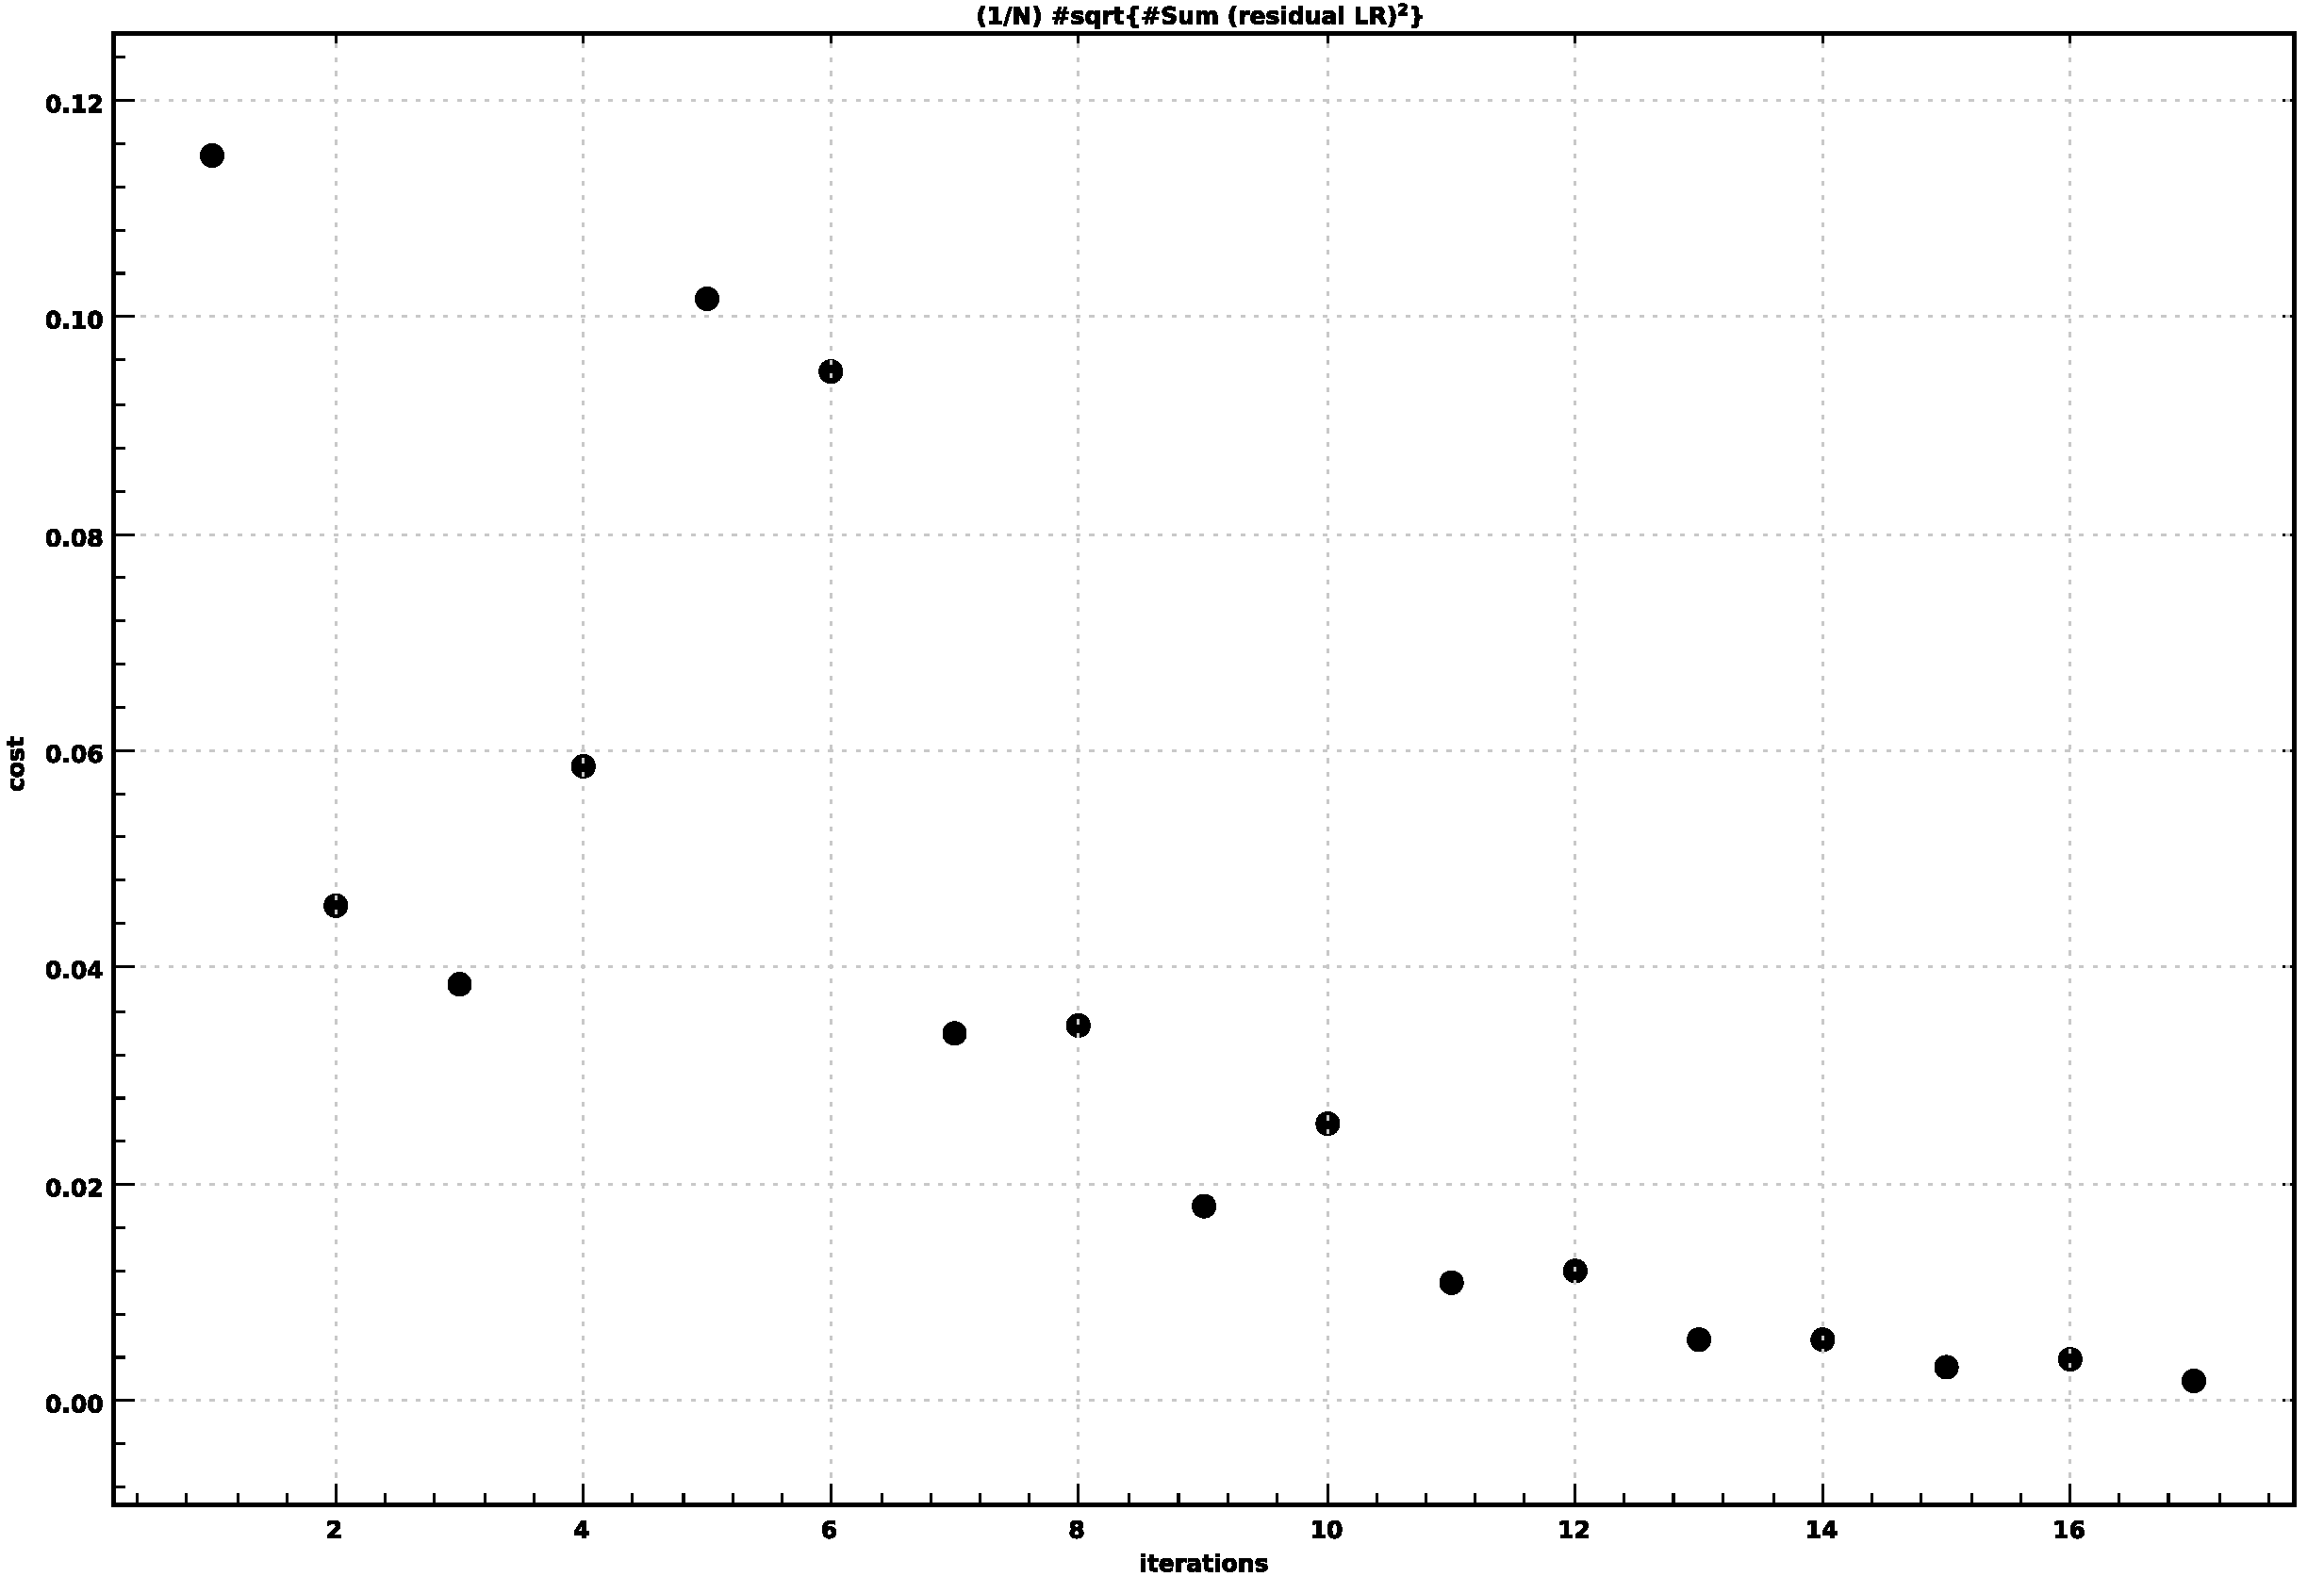
\includegraphics[width=\linewidth]{figures/conv-criteria-over-iterations.pdf}
    \end{minipage}
    
\end{frame}

\begin{frame}{Updates}
    \begin{itemize}
        \item Example: initial distributions per layer (no alignment, $\alpha = 0 ^\circ$)
        %\item At the end the minimize the 
    \end{itemize}

    \vspace{0.2cm}
    \centering
    \begin{minipage}{0.7\textwidth}
        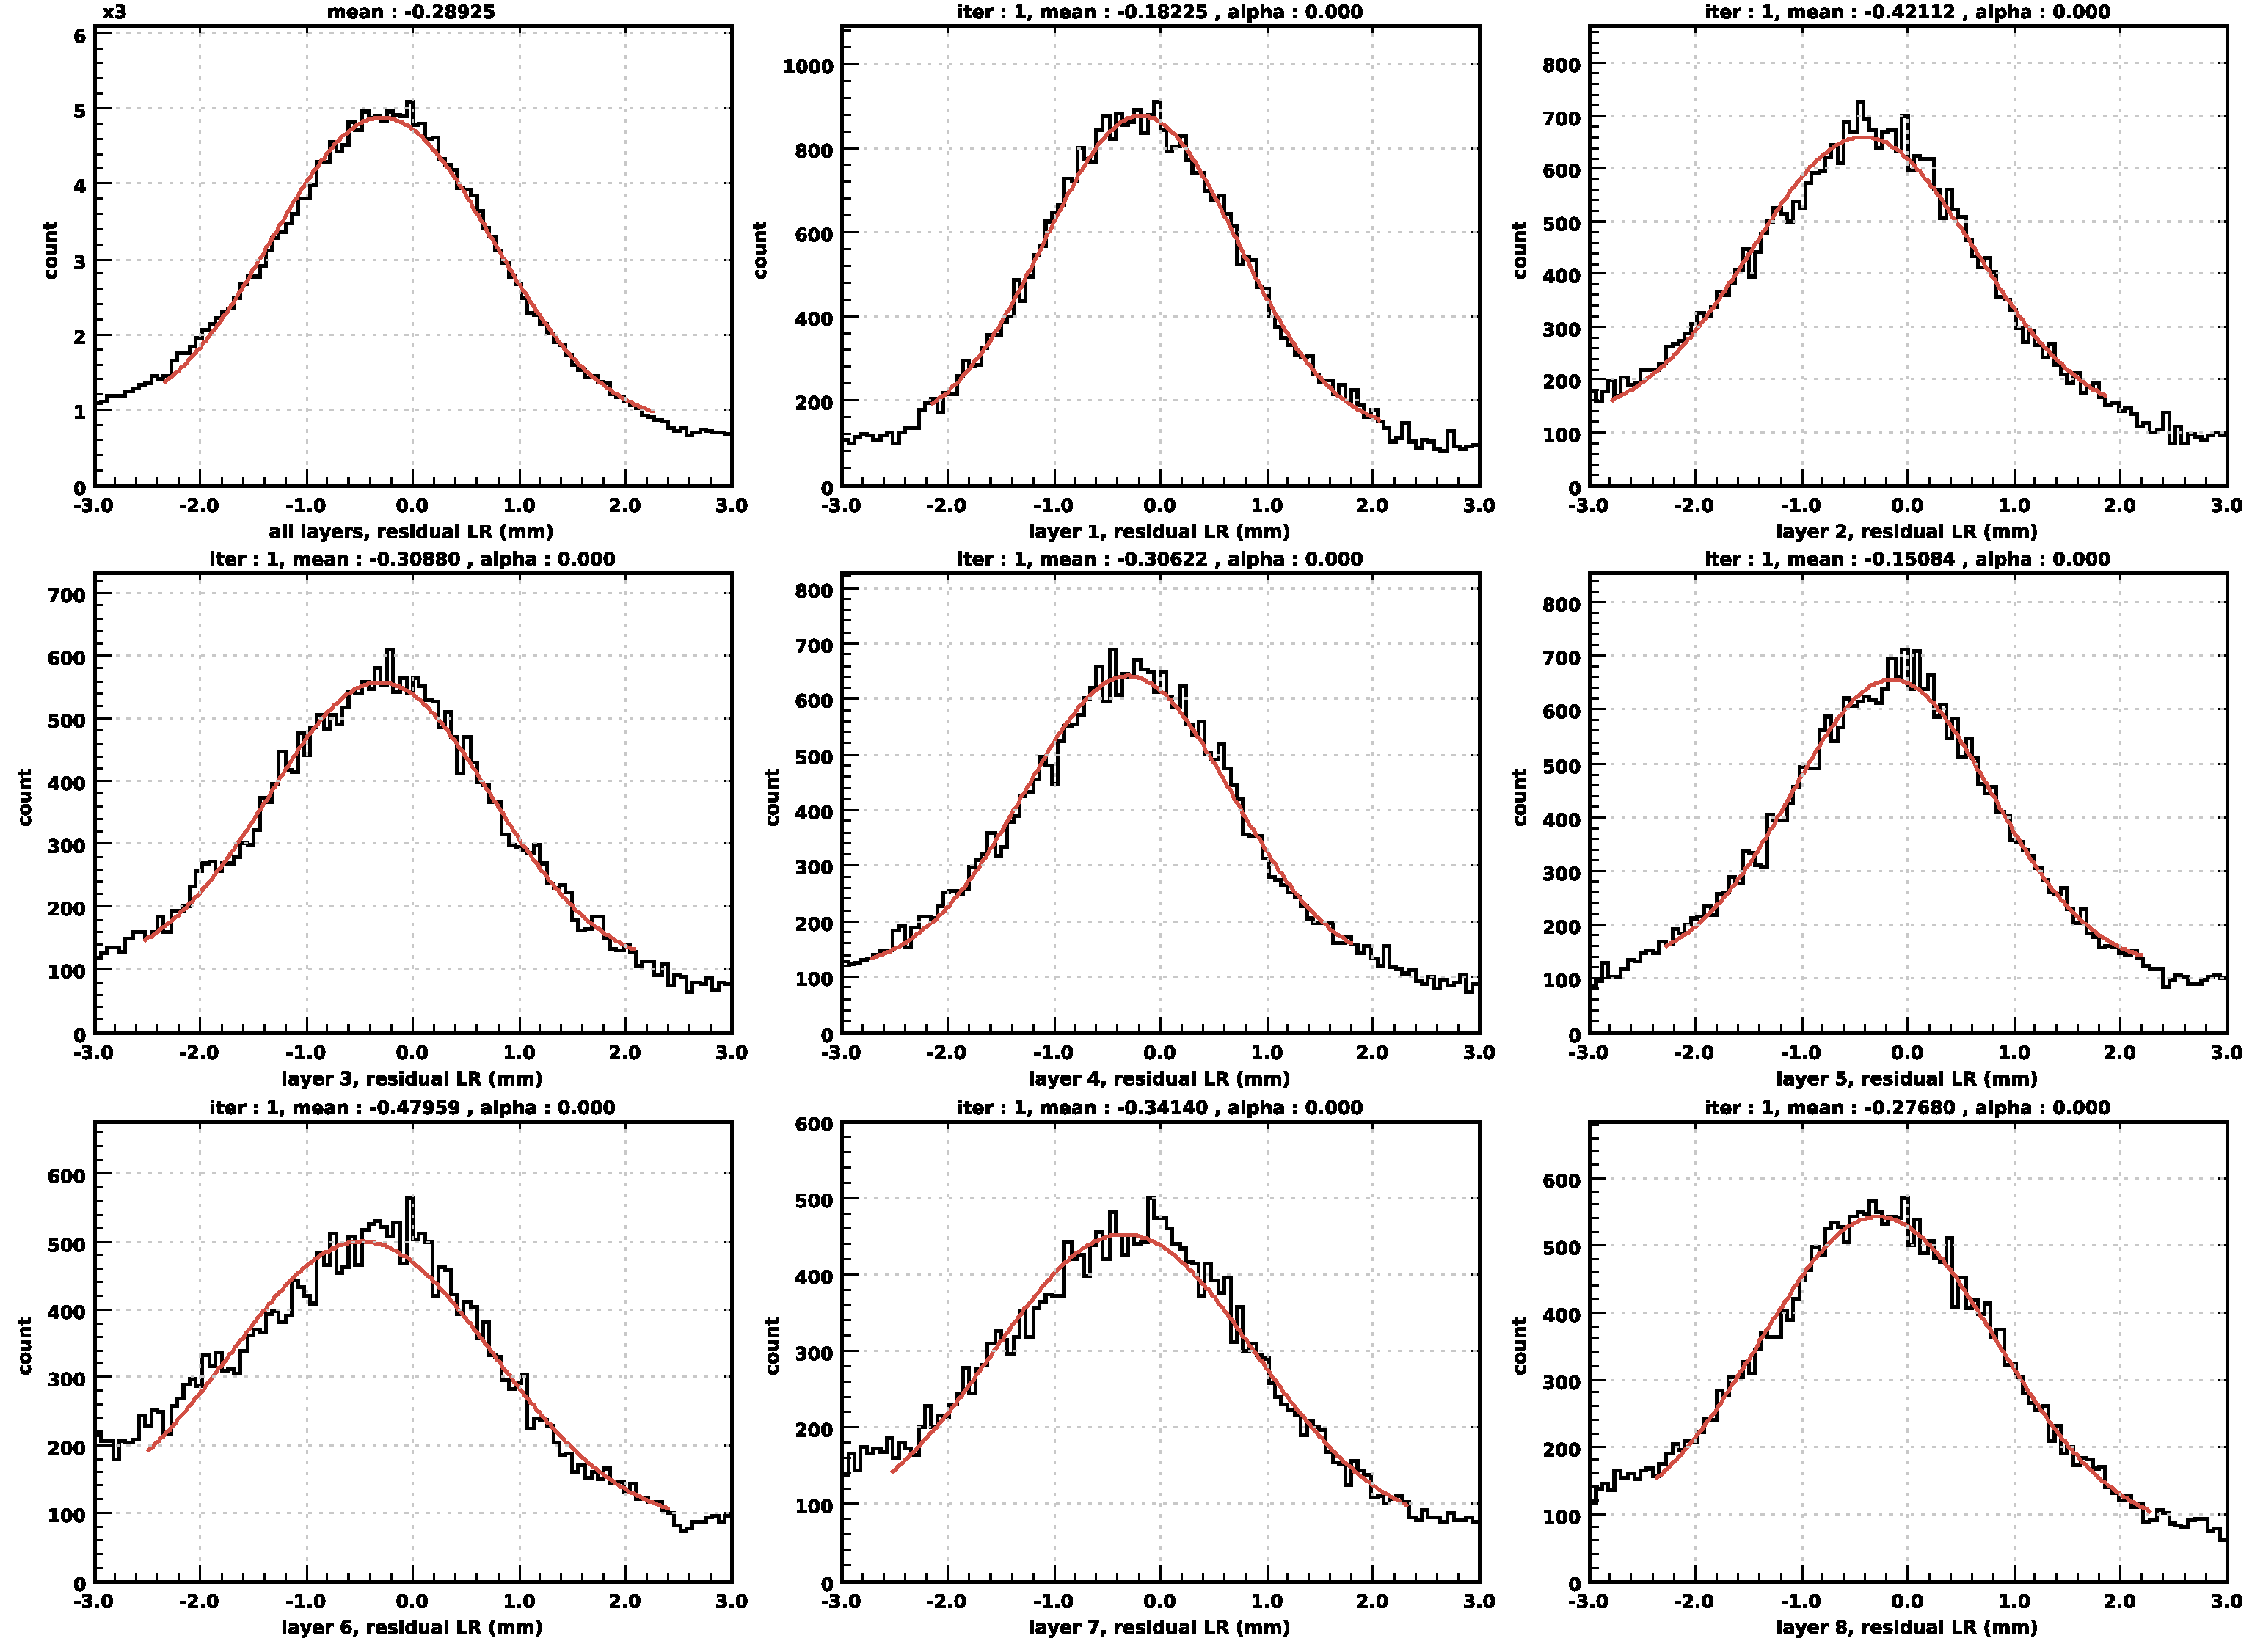
\includegraphics[width=\linewidth]{figures/residual_LR_iter_1.pdf}
    \end{minipage}
    
\end{frame}

\begin{frame}{Updates}
    \begin{itemize}
        \item Example: final distributions per layer for:  criteria $< 2 \cdot 10^{-3}$ mm
        %\item At the end the minimize the 
    \end{itemize}

    \vspace{0.2cm}
    \centering
    \begin{minipage}{0.7\textwidth}
        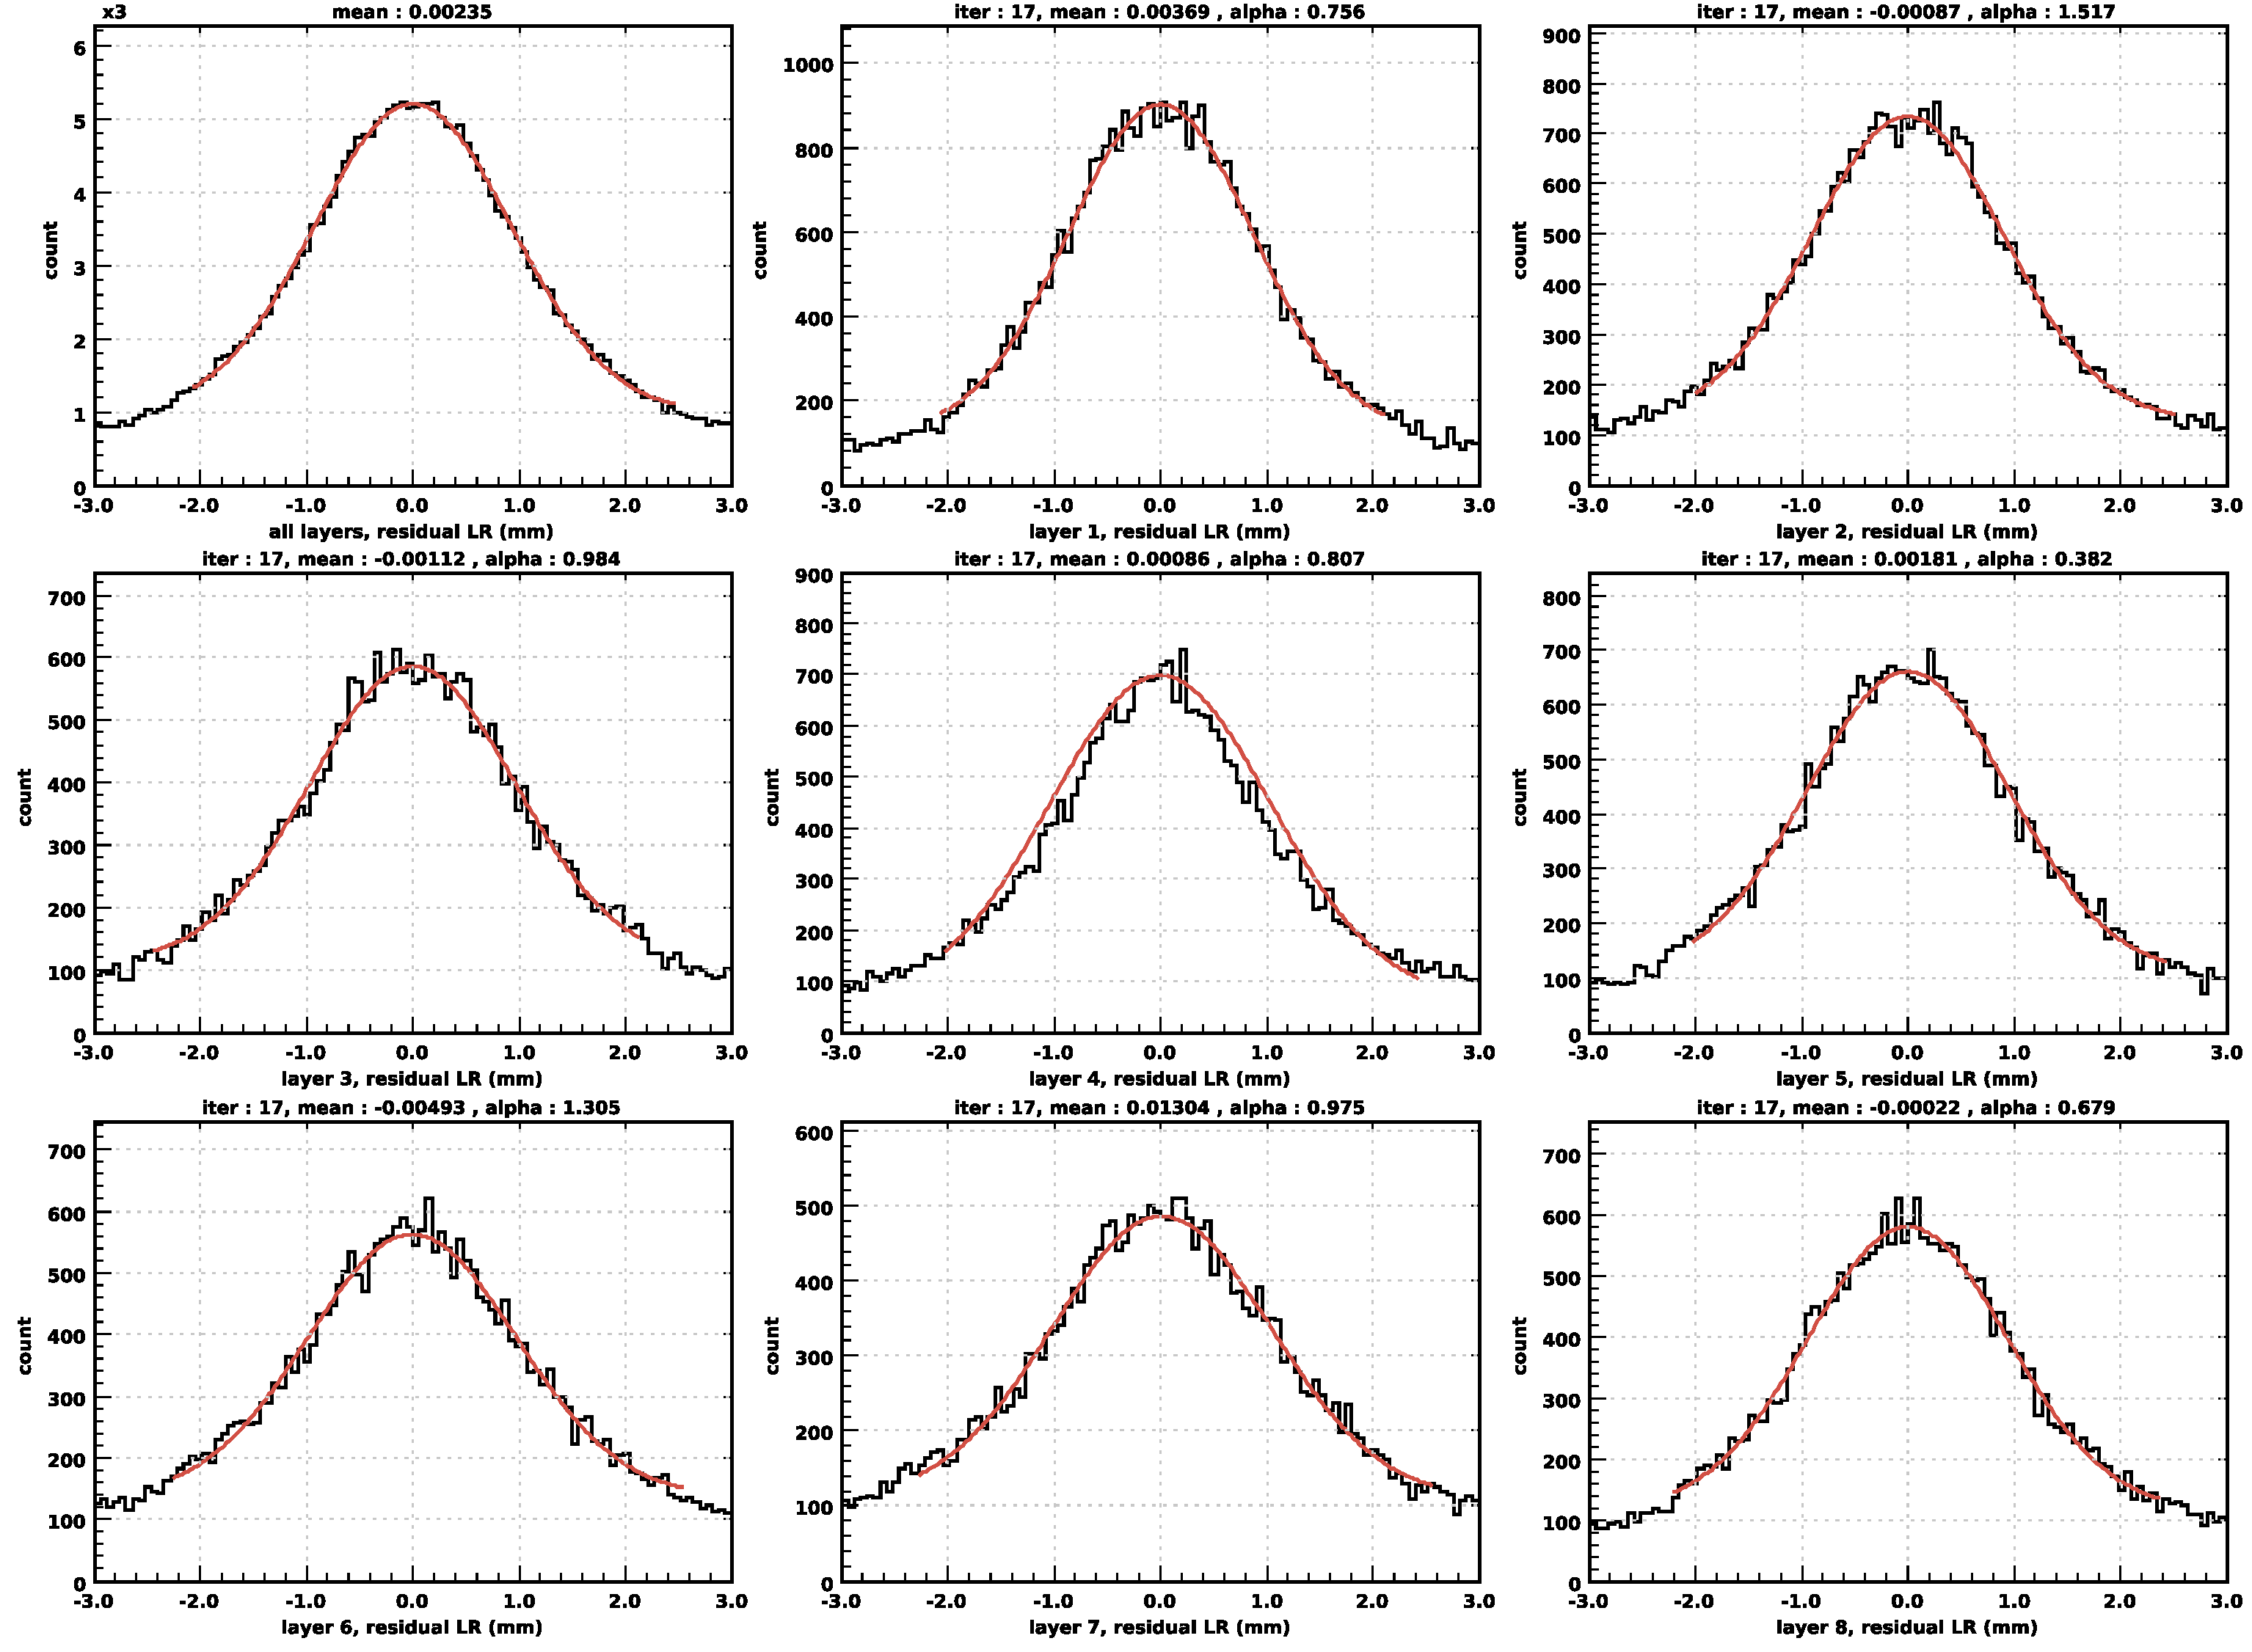
\includegraphics[width=\linewidth]{figures/residual_LR_iter_17.pdf}
    \end{minipage}
    
\end{frame}

\begin{frame}{Observation}
    \begin{itemize}
        \item Detector position with respect to CLAS
        \item The numbers inside the table are the rotation angles in deg
    \end{itemize}

    \begin{center}
        \begin{tabular}{c|c|c|c}
            AHDC position & -54 mm $^($\footnote{hand made}$^)$ & -30 mm & -70 mm\\
            \hline
            layer 11 & 0     & -1.49 & +0.756 \\
            layer 21 & +2.55 & +3.82 & +1.517 \\
            layer 22 & +2.11 & +3.24 & +0.984 \\
            layer 31 & 0     & -1.54 & +0.807 \\
            layer 32 & -0.32 & -1.96 & +0.382 \\
            layer 41 & +3.0  & +3.73 & +1.305 \\
            layer 42 & +2.13 & +3.3  & +0.975 \\
            layer 51 & -0.21 & -1.61 & +0.679 \\
        \end{tabular}
    \end{center}
    
    
\end{frame}



\begin{frame}{Backup slides}
    \begin{itemize}
        \item Procedure:
            \begin{enumerate}
                \item We looked at elastic events : electron + track (here: collection of hits only)
                \item We computed the theoretical momentum vector of the track $\vec{p}$
                \item We made the propagation without doing any fit (i.e no KF correction)
                \item We looked at {\color{blue} residual\_LR} (left-right) $\longrightarrow$ sensitive to the alignment
            \end{enumerate}
    \end{itemize}
    

    \vspace{0.2cm}
    \centering
    \begin{minipage}{0.5\textwidth}
        \includegraphics[width=\linewidth]{figures/build/illustration_residual_type.pdf}
    \end{minipage}

\end{frame}



% \begin{frame}{ATOF hit work completed 2/2}
%     \begin{itemize}
%         \item Status of the theta reconstruction
%         \item We have two peaks in the last version of the theta reconstruction
%             \begin{itemize}
%                 \item The first peak are tracks without ATOF matches
%                 \item The second peak around 86$^\circ$ are tracks with ATOF matches (45 \%)
%             \end{itemize}
%         \item The final 45 \% matches (over the nb. tracks) is low; it is essentially due the current misalignment between the AHDC and ATOF
%     \end{itemize}

%     \vspace{0.5cm}

%     \centering
%     \begin{minipage}{0.32\textwidth}
%         
\includegraphics[width=\linewidth]{figures/data_theta_new_geometry.pdf}
%     \end{minipage}
%     \begin{minipage}{0.32\textwidth}
%         
\includegraphics[width=\linewidth]{figures/data_theta_ai_matching.pdf}
%     \end{minipage}
%     \begin{minipage}{0.32\textwidth}
%         
\includegraphics[width=\linewidth]{figures/data_theta_proj_based_matching.pdf}
%     \end{minipage}







\end{document}


